\documentclass[conference]{IEEEtran}
\usepackage{graphicx,cite,bm,psfrag,amsmath}
\def\mmax{\mathop{\mbox{\scriptsize max}}}
\usepackage{float}
\def\argmin{\mathop{\mbox{arg\,min}}}
\def\argmax{\mathop{\mbox{arg\,max}}}
\newcommand{\defequal}{\stackrel{\mathrm{def}}{=}}
\renewcommand{\vec}[1]{{\ensuremath{\boldsymbol{#1}}}}
\newcommand{\popt}{\ensuremath{P^{(K)}_{opt}}}
\IEEEoverridecommandlockouts
\pagestyle{plain}
\usepackage{amsfonts}
\usepackage{algorithm, algorithmic}
\renewcommand{\algorithmicrequire}{ \textbf{Input:}} %Use Input in the format of Algorithm
\renewcommand{\algorithmicensure}{ \textbf{Procedures:}} %UseOutput in the format of Algorithm
% correct bad hyphenation here
%\hyphenation{op-tical net-works semi-conduc-tor}
\usepackage{CJK}
\usepackage{color}
\usepackage{url}
\usepackage{geometry}
\geometry{left=0.63in, right=0.81in, top=0.75in, bottom=0.75in}

\setlength{\columnsep}{0.2 in}
\begin{document}

\title{PAPR-Aware Beam Division Multiple Access for mmWave Massive MIMO Systems}
\author{\IEEEauthorblockN{Guanchong Niu and Man-On Pun\IEEEauthorrefmark{3}
%\IEEEauthorrefmark{3},
\IEEEauthorblockA{
School of Science and Engineering\\
The Chinese University of Hong Kong, Shenzhen\\
Shenzhen, Guangdong, China, 518172
\thanks{This work was supported, in part, by the CUHKSZ President's Fund under Grant No. PF.01.000211, the Shenzhen Science and Technology Innovation Committee under Grant No. ZDSYS20170725140921348 and the National Natural Science Foundation of China under Grant No. 61731018.} \thanks{\IEEEauthorrefmark{3} Corresponding author, email: SimonPun@cuhk.edu.cn.}}}}


\maketitle \thispagestyle{plain}
\pagenumbering{gobble}



\begin{abstract}
Beam division multiple access (BDMA) has recently been proposed for massive multiple-input multiple-output (MIMO) systems by simultaneously transmitting multiple users' data streams via different beams. Despite its many advantages, BDMA may suffer from a larger peak-to-average-power ratio (PAPR) as the number of transmit antennas increases. In this work, we propose to explicitly incorporate the PAPR constraints into the BDMA design by jointly performing hybrid analog-digital precoding and user-beam scheduling. More specifically, the proposed scheme designs the digital precoder with explicit PAPR constraints. In addition, to facilitate the hybrid precoder design, the proposed scheme opportunistically schedules users who are near orthogonal in the analog beam domain. To efficiently compute the optimal hybrid precoder and user-beam scheduling, we develop a greedy algorithm that first opportunistically selects users before their corresponding hybrid precoders are derived with explicit PAPR constraints. Simulation results confirm the effectiveness of proposed PAPR-aware BDMA scheme.
\end{abstract}


\section{introduction}
To meet the ever-increasing demand of higher user data rates, it is envisioned that the next-generation cellular systems will be equipped with massive antenna arrays \cite{boccardi2014five}. Capitalizing on the large number of antennas at the base-station (BS), beam division multiple access (BDMA) has recently been proposed to transmit multiple users' data streams via different beams \cite{sun2015beam, Jiang2018}. In contrast to the more conventional multiple access schemes such as Code Division Multiple Access (CDMA) or Orthogonal Frequency Multiple Division Access (OFDMA) that multiplex users in code, time and frequency domains, BDMA separates users in the beam space by transmitting data to different users in orthogonal beam directions. In \cite{sun2015beam}, BDMA was first proposed to decompose the multiuser multiple-input multiple-output (MU-MIMO) system into multiple single-user MIMO channels by multiplexing multiple users' data onto non-overlapping beams. More recently, joint user scheduling and beam selection for BDMA was formulated under the Lyapunov-drift optimization framework before the optimal user-beam scheduling policy was derived in a closed form \cite{Jiang2018}.

\begin{figure}[h]
    \begin{center}
	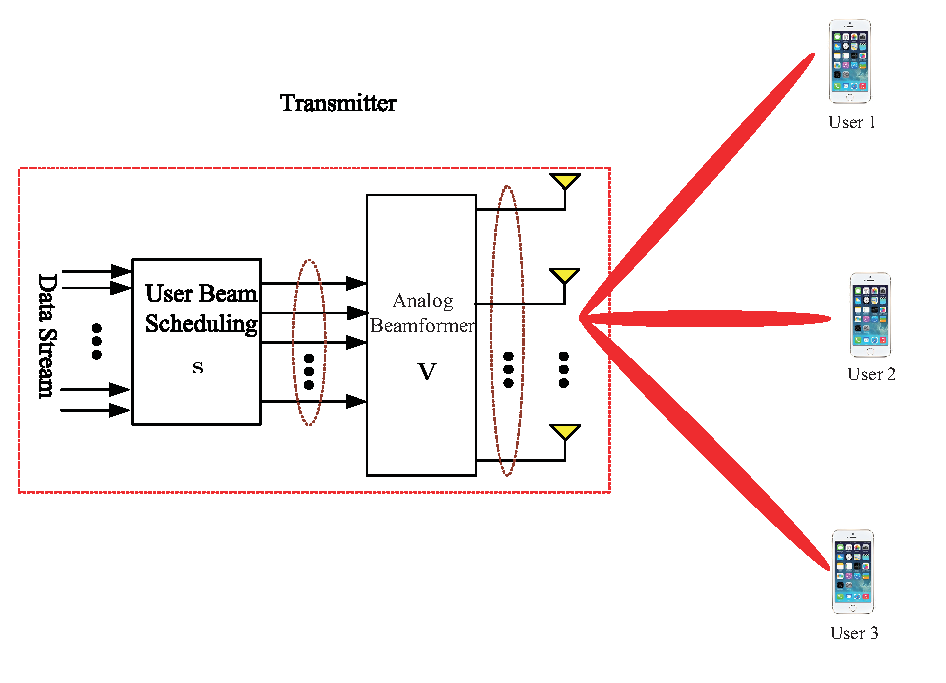
\includegraphics[scale=0.55]{Figure/BDMA.eps}
	\caption{Beam division multiple access (BDMA)}\label{fig:BDMA}
    \end{center}
\end{figure}

\begin{figure*}[ht]
    \begin{center}
	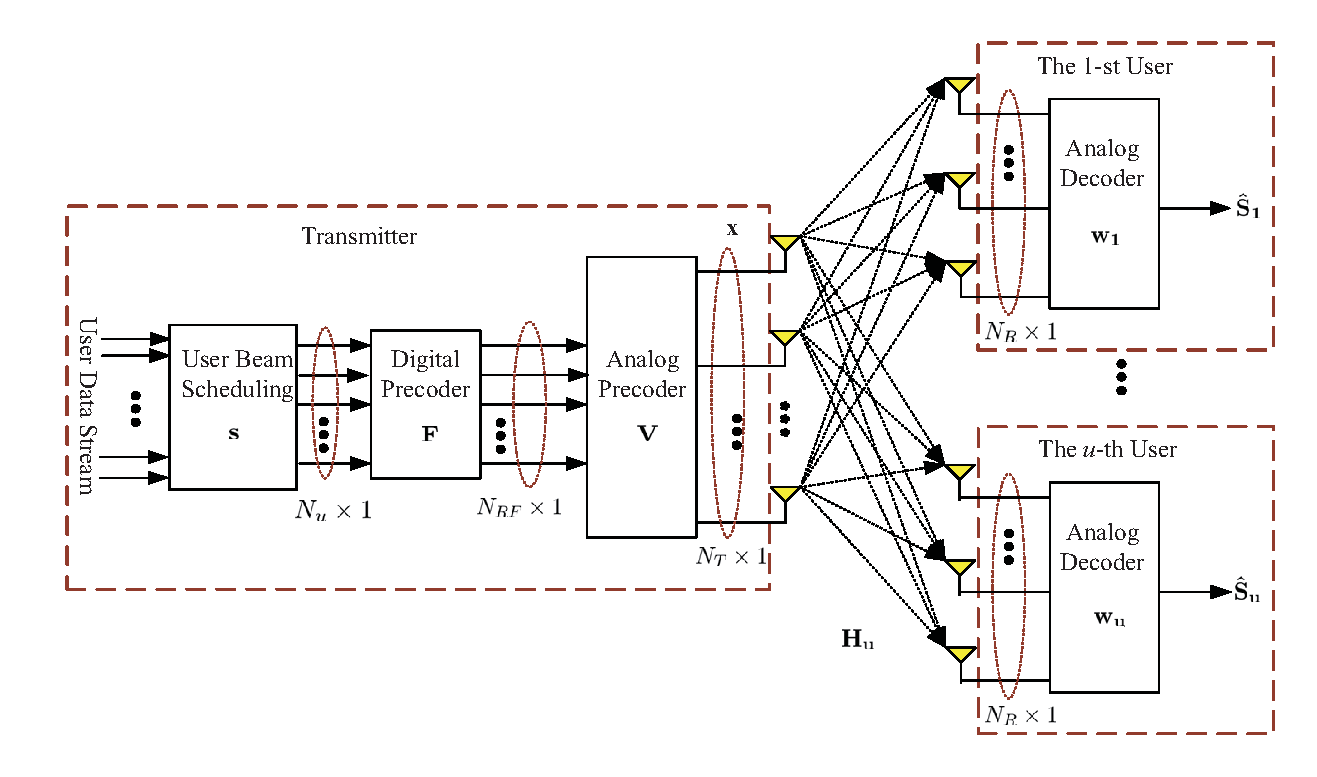
\includegraphics[scale=0.65]{Figure/SystemSchematic_new.eps}
	\caption{Schematic diagram of the hybrid precoding system under consideration}\label{fig:BlockDiagram}
    \end{center}
\end{figure*}

In the meantime, hyrbid digital and analog beamforming has also been developed for millimeter wave (mmWave) massive MIMO transmissions by dividing the procoding process into two steps, namely analog and digital precoding \cite{han2015large, el2014spatially}. More specifically, the transmitted signals are first precoded digitally using a smaller number of radio frequency (RF) chains followed by the analog precoding implemented with a much larger number of low-cost phase shifters. As a result, the hybrid analog-digital precoding architecture requires significantly less RF chains as compared to the fully digital precoding in which every available antenna element is supported by one RF chain. The hybrid precoded massive MIMO system can benefit from the interference suppression provided by the digital precoding while harvesting large antenna beamforming gains by exploiting the massive antennas available in the systems. By carefully designing the analog and digital precoders, the hybrid precoding technique has been shown to achieve throughput performance comparable to the fully digital precoding at a much lower cost\cite{alkhateeb2014channel}. Furthermore, by exploiting the vast vacant spectrum available at radio frequencies (RF) of $6$ GHz or above, mmWave MIMO systems equipped with the hybrid precoding are expected to support Gbps-order data throughput. However, since the output signals at the digital precoder are linear mixtures of multiple input data streams, the peak power after the digital precoder can theoretically ramp up to $M$ folds larger than the average power level with $M$ being the number of data streams. Therefore, a large $M$ can potentially incur large peak-to-average power ratio (PAPR) problem \cite{mohammed2013per,Chen2017}, which in turn requires expensive linear power amplifiers (PAs) to avoid signal spectral spreading and in-band distortion.

\setlength{\columnsep}{0.5 in}
In this work, we propose to employ BMDA as the multiple access scheme for mmWave massive MIMO systems as the mmWave channels are shown to have very limited scattering paths. Furthermore, we adopt the hybrid precoding in designing the analog beams. Since multiuser interference in BDMA-based massive MIMO systems are handled by both analog beamforming in the beam domain and digital precoding through zero-forcing interference cancelation at the same time, the proposed scheme has more degrees of freedom in handling other system impairments such as PAPR. More specifically, we propose PAPR-aware BDMA for mmWave massive MIMO systems by jointly performing hybrid analog-digital precoding and user-beam scheduling with explicit PAPR constraints. In principle, since these two tasks of precoding design and user-beam scheduling are coupled, the optimal hybrid precoder and user-beam scheduling can be found only after all combinations of scheduled users are exhaustively examined. To cope with the prohibitively expensive computational complexity mentioned above, a greedy algorithm is devised to opportunistically and efficiently select users whose array response vectors are nearly orthogonal in the beam domain while the digital precoder is designed to suppress the residual multiuser interference as well as PAPR.

\setlength{\columnsep}{1 in}
Compared to the existing BDMA works \cite{sun2015beam, Jiang2018}, our proposed BDMA scheme can achieve multiuser interference-free {\em without} requiring perfectly orthogonal beams as residual interference can be removed by digital precoding. Furthermore, unlike the conventional hybrid precoding proposed in \cite{alkhateeb2014channel}, the proposed digital precoder is designed to handle both multiuser interference and PAPR while multiuser interference is also suppressed by the analog precoder in the beam domain through user scheduling. Computer simulation is used to confirm the performance of the proposed PAPR-aware BDMA scheme.

\setlength{\columnsep}{1 in}
{\underline{Notation}: Vectors and matrices are denoted by boldface letters. ${\bm A}^T$ and ${\bm A}^H$ denote transpose and conjugate transpose of ${\bm A}$, respectively. $\bm{A}^\dagger$ being the pseudo inverse of $\bm{A}$ while $||\bm{A}|| $ and $|\bm{A}|$ stand for the Frobenius norm and determinant of ${\bm A}$, respectively. $\bm{A}(i,j)$ denotes the $i$ row, $j$ column element of ${\bm A}$; $|\cal{I}|$ is the cardinality of the enclosed set ${\cal I}$; Finally, $\mathbb{E}[ \cdot] $ and $\Re\{\cdot\}$ denote the expectation and real part of a random variable.}


\section{System model and problem formulation}

\subsection{System Model}

We consider a multi-user mmWave MIMO system shown in \figurename{ \ref{fig:BlockDiagram}}, in which a transmitter equipped with $N_{RF}$ RF chains and $N_T$ antennas transmits $N_U$ data streams to $N_U$ receivers with $N_R$ receive antennas. Following the same assumption commonly employed in the literature \cite{alkhateeb2015limited}, we assume only one data stream is designated to each scheduled receiver. We use ${\bm s}(n)$ to denote the $n$-th block of $N_U$ data to be transmitted with $\mathbb{E}\left[\bm{ss}^H\right]=\frac{1}{N_U}\bm{I}_{N_U}$. In the sequel, we concentrate on a single block and omit the temporal index $n$ for notational simplicity.


The hybrid precoding system first multiplies ${\bm s}$ with the digital precoding matrix $\bm{F}=\left[{\bm f}_1,\cdots,{\bm f}_u,\cdots{\bm f}_{N_U}\right]$ with ${\bm f}_u$ of dimension $N_{RF}\times 1$ being the digital beamforming vector for the $u$-th user, $u=1,2,\cdots,N_U$. After that, the output signal will be multiplied by the analog precoding matrix $\bm{V}=\left[{\bm v}_1,\cdots,{\bm v}_i,\cdots,{\bm v}_{N_{RF}}\right]$ with ${\bm v}_i$ of dimension $N_T\times 1$ being the $i$-th analog beamforming vector for $i=1,2,\cdots,N_{RF}$. The resulting precoded signal $\bm x$ of dimension $N_T\times 1$  can be expressed as

\begin{equation}{\label{eq:transx1}}
{\bm x} = \bm{V}\cdot \bm{F}\cdot\bm{s}= \bm{V}\sum_{u=1}^{N_U}\bm{f}_us_u
\end{equation}

The precoded signal $\bm x$ is then broadcast to $N_U$ users. The signal received by the $u$-th user is given by

\begin{eqnarray}{\label{eq:transx2}}
{\bm y}_u &=& \bm{H}_u \bm{x} + \bm{n}_u\\
&=&\bm{H}_u \bm{V}\bm{f}_us_u+\bm{H}_u \bm{V}\sum_{\substack{i=1 \\ i\neq u}}^{N_U}\bm{f}_is_i+\bm{n}_u,
\end{eqnarray}
where $\bm{H_u}$$\in\mathbb{C}^{N_R\times N_T}$ is the MIMO channel matrix between the transmitter and the $u$-th receiver\cite{el2014spatially}. Furthermore, $\bm{n}_u$ is complex additive white Gaussian noise with zero mean and variance equal to $\sigma^2$.

Assuming the receivers are all low-cost terminals that perform analog beamforming only in decoding, the decoded signal by the $u$-th user denoted by $\hat{s}_u$ is given by
\begin{equation}{\label{eq:hats}}
\hat{s}_u = \bm{w}_u^H \bm{H}_u \bm{V} \bm{f}_{u} \bm{s} + \bm{w}_u^H \bm{\tilde{n}}_u,
\end{equation}
where ${\bm w}_u$ of dimension $N_T\times 1$ is the analog beamforming vector employed by the $u$-th receiver with the power constraint of $|\bm{w}_u|^2=1$ and
\begin{equation}
\bm{\tilde{n}}_u=\bm{H}_u \bm{V}\sum_{\substack{i=1 \\ i\neq u}}^{N_U}\bm{f}_is_i+\bm{n}_u.
\end{equation}
Note that the first term in Eq.~(\ref{eq:hats}) stands for the desired signal while the second term is the sum of its own receiver noise and interference from other users.

\subsection{Channel Model}
As shown in \cite{rappaport2014millimeter}, the mmWave wireless channel can be well modeled by the Saleh-Valenzuela model. Following the same approach developed in \cite{alkhateeb2014channel}, we assume that each scatter only contributes one single propagation path. As a result, the $u$-th user's channel model can been modeled as:
\begin{equation}{\label{eq:Hu}}
\bm{H}_u = \sqrt{\frac{N_{T}N_{R}}{L_{u}}}\sum_{l=1}^{L_u}\alpha_{u,l}\cdot \bm{a}_{R}(\phi^r_{u,l},\theta^r_{u,l}) \cdot\bm{a}_{T}^{H}(\phi^t_{u,l},\theta^t_{u,l}),
\end{equation}
where $L_u$ is the number of scatters of the $u$-th user's channel. Furthermore, $\alpha_{u,l}$, $\theta^r_{u,l}/\phi^r_{u,l}$ and $\theta^t_{u,l}/\phi^t_{u,l}$ are the complex path gain, azimuth/elevation angles of arrival(AoA) and azimuth/elevation angles of departure(AoD) of the $l$-th path of the $u$-th user, respectively. Finally, ${\bm a}$ is the array response vector. For an uniform planar array (UPA) of size $P\times Q$ considered in this work, the array response vector ${\bm a}$ is given by \cite{alkhateeb2014channel}
\begin{flalign}\label{eq:UPAvec1}
&\bm{a}(\phi,\theta) =\frac{1}{\sqrt{N_T}}\left[1,  e^{jkd(\sin\phi \sin\theta +\cos\theta)},\cdots,\right.&&\nonumber\\
&\left. e^{jkd\left(p\sin\phi \sin\theta +q\cos\theta\right)},\cdots, e^{jkd\left((P-1)\sin\phi \sin\theta +(Q-1)\cos\theta\right)}\right]^T,&&
\end{flalign}
where $k=\frac{2\pi}{\lambda}$ is the wavenumber while $d$ is the distance between two adjacent antennas.

In mmWave communications, due to the high path loss and atmospheric absorption, it is common to assume that the channel is dominated by one line-of-sight (LoS) path, i.e. $L_u=1$ for all users \cite{alkhateeb2014channel}. Under such an assumption, the channel model in Eq.~(\ref{eq:Hu}) can be further simplified as
\begin{equation}{\label{eq:HuLu1}}
	\bm{H}_u = \sqrt{N_{T}N_{R}}\cdot\alpha_u \cdot\bm{a}_{R}(\phi^r_{u},\theta^r_{u})\cdot\bm{a}^{H}_{T}(\phi^t_{u},\theta^t_{u}).
\end{equation}

\subsection{Problem Formulation}
For notational simplicity, we denote by ${\bm{g}}_{u}^H$ the effective array gain of the $u$-th user with
\begin{equation}\label{eq:defgu}
{\bm{g}}_{u}^H = \bm{w}^H_u \bm{H}_u \bm{V}.
\end{equation}

Then, the channel capacity of the $u$-th user is given by
\begin{equation}\label{eq:6}
	R_u = \log\left(1+\frac{\frac{P}{N_U}|{\bm{g}}_{u}^H \bm{f}_u|^2}{\frac{P}{N_U}\displaystyle\sum_{\substack{i=1 \\ i\neq u}}^{N_U}|{\bm{g}}_{u}^H\bm{f}_i|^2+\sigma^2}\right).
\end{equation}
Subsequently, the system sum-rate capacity that is a function of ${\bm V}$ and ${\bm F}$ can be computed as
\begin{equation}
R_{tot}=\sum_{u=1}^{N_U}R_u.
\end{equation}

Finally, the optimal design of the digital and analog precoding matrices can be formulated as
\begin{align}\label{eq:maxsumrate}
\left\{{\bm V}^*,{\bm F}^*\right\} &= \argmax_{\tilde{\bm V},\tilde{\bm F}} R_{tot}\left(\tilde{\bm V},\tilde{\bm F}\right)\\ \nonumber
s.t. \quad&||\tilde{\bm V}\tilde{\bm f}_u||^2 = 1, \quad u=1,2,\cdots,N_U.
\end{align}

\section{Proposed PAPR-Aware Hybrid Beamforming}
\subsection{PAPR Reduction via Convex Optimization}
For the single-path LoS environment considered in this work, the channel matrix of the $u$-th user is well structured as given by Eq.~\eqref{eq:HuLu1}. Subsequently, the optimal analog precoding at the transmitter is given by ${\bm v}^*_u = {\bm a}_T\left(\phi^t_u,\theta^t_u\right)$ while the optimal analog beamforming vector at the receiver is given by ${\bm w}^*_u = {\bm a}_R\left(\phi^r_u,\theta^r_u\right)$\cite{alkhateeb2014channel}. Assuming that the transmitter has perfect channel state information (CSI), then all AoA and AoD information, {\em i.e.} $\left\{\phi^t_u,\theta^t_u,\phi^r_u,\theta^r_u\right\}$, is perfectly known to the transmitter. As a result, the optimization problem in Eq.~(\ref{eq:maxsumrate}) can be simplified as
\begin{flalign}\label{eq:optdigPreMat}
{\bm F}^* &= \argmax_{\tilde{\bm F}} R_{tot}\left({\bm V}^*,\tilde{\bm F}\right)\\
s.t. \quad&||{\bm V}^*\tilde{\bm f}_u||^2 = 1 , \quad u=1,2,\cdots,N_U.\nonumber
\end{flalign}

We denote by $\hat{\bm s}=\left[\hat{s}_1,\hat{s}_2,\cdots,\hat{s}_{N_U}\right]^T$ the estimated signal vector. Recalling Eq.~(\ref{eq:hats}), $\hat{\bm s}$ can be expressed as \cite{alkhateeb2014channel}
\begin{equation}\label{eq:hatsAllUsers}
\hat{\bm s} = {\bm G}\cdot \bm{F} \cdot\bm{s} + \bm{\xi},
\end{equation}
where ${\bm G}=\left[{\bm g}_1,{\bm g}_2,\cdots,{\bm g}_{N_U}\right]^H$ is of dimension $N_U\times N_{RF}$ and ${\bm \xi}=\left[{\bm w}_1^H\tilde{\bm n}_1,{\bm w}_2^H\tilde{\bm n}_2,\cdots,{\bm w}_{N_U}^H\tilde{\bm n}_{N_U}\right]^T$. \cite{alkhateeb2014channel} proposed a zero-forcing approach to solve Eq.~(\ref{eq:optdigPreMat}) by setting
\begin{equation}\label{eq:ZFU-HBF}
\bm{F}_{ZF}={\bm G}^\dagger = \bm{G}^H(\bm{G}\bm{G}^H)^{-1},
\end{equation}
with $N_{RF}\geq N_U$.

To satisfy the power constraint, power normalization is performed on each ${\bm f}_u$ derived from $\bm{F}_{ZF}=\left[\bm{f}_{ZF,1},\bm{f}_{ZF,2},\cdots,\bm{f}_{ZF,N_U}\right]$ as
\begin{equation}\label{eq:ZFU-HBF}
\bm{f}^*_{ZF,u} = {\frac{\bm{f}_{ZF,u}}{||\bm{V}\cdot\bm{f}_{ZF,u}||}}.
\end{equation}
In the sequel, the hybrid beamforming scheme derived from Eq.~(\ref{eq:ZFU-HBF}) is referred to as the unconstrained zero-forcing hybrid beamforming (ZFU-HBF) for benchmarking our following proposed schemes.

Since the zero-forcing solution $\bm{F}_{ZF}$ is designed without taking into account the PAPR concerns, the output signal from the digital precoder $\bm{F}_{ZF}$ may suffer from a peak power much larger than its average power level. To circumvent this problem, we first consider the more conventional technique by clipping the signal with a pre-set threshold $\lambda$. Mathematically, each element of $\bm{F}_{ZF}$ is passed through the following filter, for $i=1,2,\cdots, N_{RF}$ and $j=1,2,\cdots, N_{U}$.
\begin{equation}\label{eq:clipping}
 \left[\bm{F}_{ZF}\right]^{clip}_{ij}=\left\{
\begin{aligned}
& \left[\bm{F}_{ZF}\right]_{ij}, &\mbox{if}\quad |\left[\bm{F}_{ZF}\right]_{ij}|\leq\lambda \\
& \lambda, &\mbox{otherwise}  \\
\end{aligned}
\right.
\end{equation}
In the sequel, the hybrid beamforming scheme derived from Eq.~(\ref{eq:clipping}) is referred to as the zero-forcing with clipping hybrid beamforming (ZFC-HBF).

While clipping is a simple and yet effective technique for PAPR reduction, it inevitably incurs spectral spreading, in-band distortion and subsequently, performance degradation. In sharp contrast to the direct clipping, we propose to incorporate the threshold $\lambda$ into the design of ${\bm F}$. More specifically, we can formulate the optimization problem in Eq.~(\ref{eq:optdigPreMat}) as follows:
\begin{flalign}\label{eq:optdigPreMatPAPR}
{\bm F}^* &= \argmax_{\tilde{\bm F}} R_{tot}\left({\bm V}^*,\tilde{\bm F}\right)\\
s.t. \quad&||{\bm V}^*\tilde{\bm f}_u||^2 = 1 \nonumber\\
\quad &\left|\tilde{\bm f}_{u}\right|_i \leq \lambda \quad\mbox{ for } i=1,2,\cdots,N_{RF}.\nonumber
\end{flalign}
The problem in Eq.~(\ref{eq:optdigPreMatPAPR}) can be approximated by the following convex optimization problem and solved by standard optimization tools such as CVX \cite{cvx}.
\begin{flalign}\label{eq:optdigPreMatCVX}
{\bm F}^* &= \argmin_{\tilde{\bm F}} \|{\bm G}\tilde{\bm F}-{\bm{GF}_{ZF}}\|^2\\
s.t. \quad&||{\bm V}^*\tilde{\bm f}_u||^2 = 1 \nonumber\\
\quad &\left|\tilde{\bm f}_{u}\right|_i \leq \lambda \quad\mbox{ for } i=1,2,\cdots,N_{RF}.\nonumber
\end{flalign}
The amplitude of each RF chain is constrained to be $\lambda$ by solving the convex optimization problem. In the sequel, the hybrid beamforming scheme derived from Eq.~(\ref{eq:optdigPreMatPAPR}) is referred to as the PAPR-aware hybrid beamforming (PAPRA-HBF).

\subsection{PAPR Reduction via Opportunistic Scheduling}
In this section, we consider the joint optimization of analog and digital precoders by incorporating multiuser scheduling into our PAPR reduction design. This is in sharp contrast to the conventional design philosophy. As shown in most existing works \cite{alkhateeb2015limited}, the analog precoder is first optimized to provide the maximum beamforming gain by matching the user's AoD, {\em i.e.} fixing the ${\bm G}$ matrix first before designing the optimal digital precoder to suppress multiuser interference. Since these two steps are performed sequentially, it may become very challenging for the digital precoder to simultaneously suppress interference while reducing PAPR at the same time, particularly if the analog precoders entail heavy multiuser interference. Motivated by this observation, we propose to opportunistically schedule $N_U$ users whose array response vectors $\bm{a}_{T}(\phi^t_u,\theta^t_u)$ are as orthogonal as possible to each others'. As a result, this scheduling scheme will enable the digital precoder to have more degrees of freedom to reduce PAPR. More specifically, we consider scheduling $N_U$ users from $U$ active users. Since the total number of possible combinations given by $C\left(U, N_U\right)=\frac{U!}{(U-N_U)!N_U!}$ can be rather large, it may be infeasible to exhaustively search over all possible combinations to find out the most orthogonal set of $N_U$ users. To cope with this obstacle, we devise a greedy algorithm to select $N_U$ users from the $U$ active users.

\begin{algorithm}[h] 		
	\caption{Greedy scheduling algorithm for PAPR-aware hybrid beamforming}
	\label{selection}
	\begin{algorithmic}
		\REQUIRE  \quad
		\STATE	All user index set: $\mathcal{X}$\\
		\STATE  Selected user index set : $\cal{I}=\emptyset$\\
		\STATE  Number of user to be selected: $N_U$
		\ENSURE   	
		\STATE Initialization: Assign the user index $x$ corresponding to the largest channel gain $|\alpha|$ to ${\cal I}$, {\em i.e.} ${\cal I} \leftarrow  x$ and ${\cal X}\setminus x$	
		\WHILE{$|{\cal I}|< N_U$}
        \STATE ${\bm A}=\left[\bm{a}_{T}\left(\phi^t_{i_1},\theta^t_{i_1}\right),\bm{a}_{T}\left(\phi^t_{i_2},\theta^t_{i_2}\right),\cdots,\bm{a}_{T}\left(\phi^t_{i_{|{\cal I}|}},\theta^t_{i_{|{\cal I}|}}\right)\right]$
        \STATE Compute the projection space: ${\bm P}_A = {\bm A}{\bm A}^{\dagger}$ 		 				
		\FOR{$x$ in {$\mathcal{X}$}}
		\STATE $p(x) = \|{\bm P}_A\cdot {\bm a}_T\left(\phi^t_{x},\theta^t_{x}\right)\|^2$ 				 								
		\ENDFOR
		\STATE  Find the user index $x^*$ with the minimum $p(x)$ 									
		\STATE	Update ${\cal I} \leftarrow  x^*$ and ${\cal X}\setminus x^*$	
		\ENDWHILE	
	\end{algorithmic}
\end{algorithm}

Denote by $\cal{I}$ the index set of the selected users. The proposed greedy algorithm first finds the user with the strongest instantaneous channel gain as the first selected user and assigns its index to $\cal{I}$ as its first element $i_1$. The array response vector of the first selected user is given by $\bm{a}_{T}\left(\phi^t_{i_1},\theta^t_{i_1}\right)$. Then, the algorithm will find a user among the remaining users whose array response vector is the most orthogonal to $\bm{a}_{T}\left(\phi^t_{i_1},\theta^t_{i_1}\right)$ and assigns its index to $\cal{I}$ as $i_2$. After that, the algorithm will construct a signal subspace spanned by $\left\{\bm{a}_{T}\left(\phi^t_{i_1},\theta^t_{i_1}\right),\bm{a}_{T}\left(\phi^t_{i_2},\theta^t_{i_2}\right)\right\}$ before projecting the array response vectors of the remaining unselected users onto the signal subspace. The user whose array response vector has the least projection power on the signal subspace will be selected as the third user and assigned to $\cal{I}$ as $i_3$. This process will continue until all $N_U$ users are selected. It should be emphasized that the proposed greedy algorithm is different from the existing opportunistic scheduling algorithms in that user selection is not completely based on instantaneous channel gains. The $N_U$ users selected by the greedy algorithm will have less multiuser interference as they are selected because of their almost orthogonal transmit array response vectors. The above greedy algorithm is summarized in {\bf Algorithm 1} Table.

Upon all $N_U$ users are selected, Eq.~(\ref{eq:optdigPreMatCVX}) can be utilized to derive the optimal digital beamforming vectors with reduced PAPR. In the sequel, the hybrid beamforming scheme proposed in {\bf Algorithm 1} Table is referred to as the PAPR-Aware {\em opportunistic} hybrid beamforming (PAPRA-OHBF).



\section{simulation results}
In this section, we use computer simulation to compare the performance of various hybrid precoding algorithms discussed above in terms of peak-to-average ratio and system sum-rate capacity. Unless specified otherwise, we consider a transmitter equipped with an $8\times 8$ UPA ({\em i.e.} $N_T=64$) and $N_{RF}=4$ RF chains serving $N_U=4$ users each equipped with a $4\times 4$ UPA ({\em i.e.} $N_R=16$). The channels are single-path with the azimuth AoAs/AoDs being uniformly distributed over $[0, 2\pi]$ and the elevation AoAs/AoDs being uniformly distributed in $[-\pi/2, \pi/2]$, respectively. For opportunistic schemes, we consider selecting the $4$ users from $20$ active users. For each computer experiment, we compute the average over 500 realizations.

\begin{figure}[ht]
	\begin{center}
	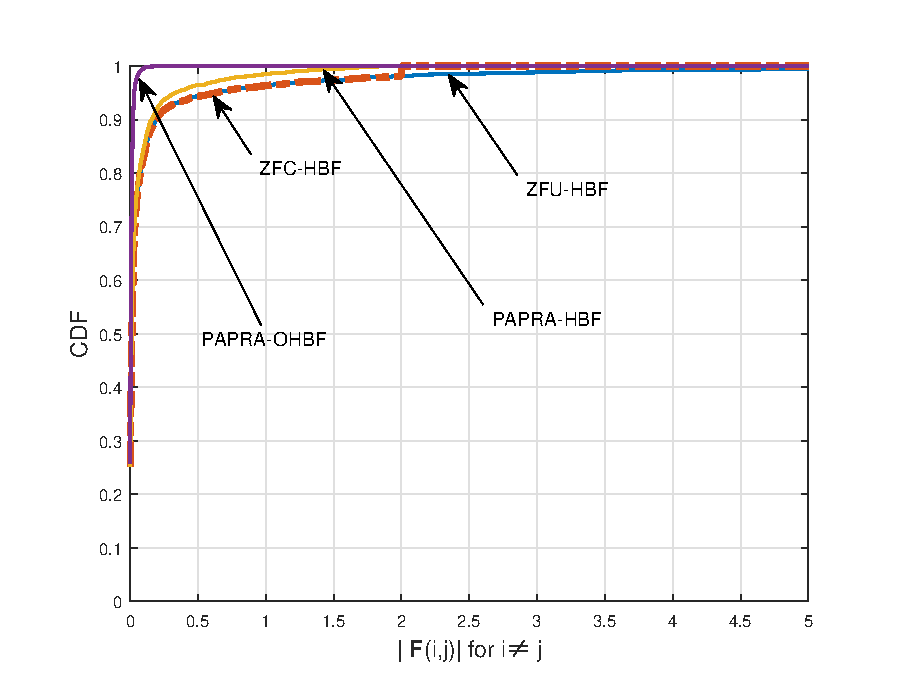
\includegraphics[width=3.8in,height=3in]{Figure/cdf2.eps}
\caption{Comparison of CDF of off-diagonal elements of the digital precoding matrix ${\bm F}$.}\label{fig:CDF}
    \end{center}
\end{figure}

We first compare the PAPR performance by investigating the cumulative distribution function (CDF) of the absolute value of the off-diagonal elements of ${\bm F}$ derived from the algorithms discussed above. Inspection of Fig.~\ref{fig:CDF} suggests that ZFU-HBF has the heaviest tail and subsequently the worst PAPR performance. Furthermore, clipping helps to eliminate all values larger than the clipping threshold, {\em $\lambda=2$}. As a result, the curve labeled as ``ZFC-HBF" has no value larger than $2$. Finally, the PAPR-aware schemes, namely ``PAPRA-HBF" and ``PAPRA-OHBF", have much thinner tails and achieve the best PAPR performance.

\begin{figure}[ht]
 	\begin{center}
 	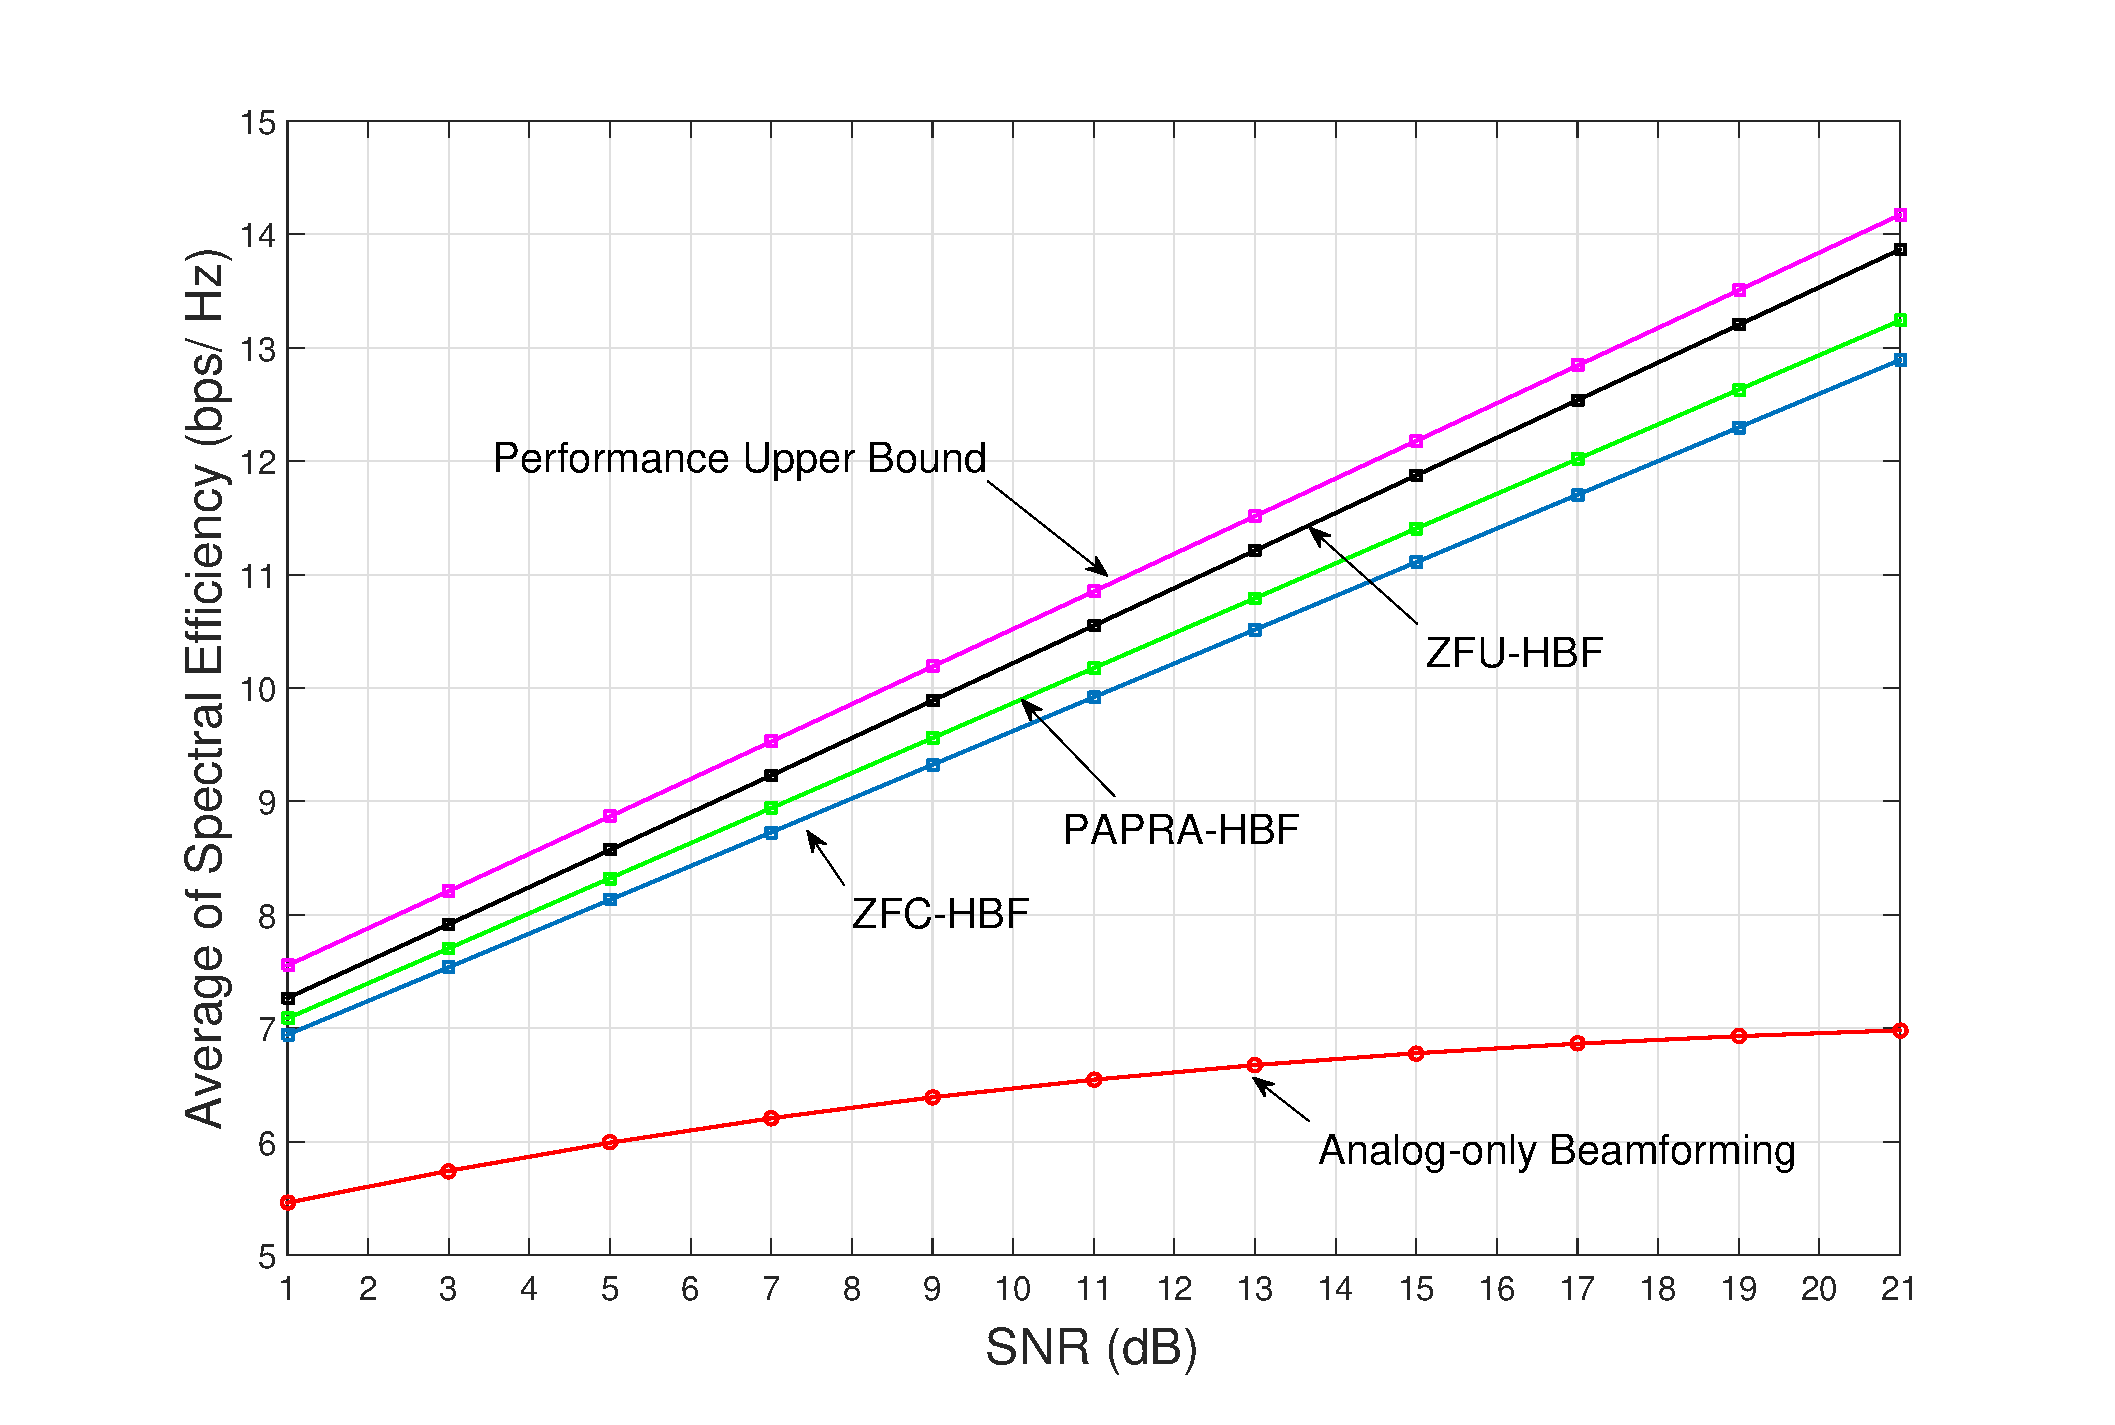
\includegraphics[width=3.8in,height=2.8in]{Figure/SpectralEffNoSelection3.eps}
 	\caption{Comparison of Sum-rate capacity for non-opportunistic schemes.}\label{fig:SpectralEffNoSelection}
    \end{center}
\end{figure}

Fig.~\ref{fig:SpectralEffNoSelection} shows the sum-rate capacity achieved by the precoding schemes considered in this work. The curve labelled as ``Performance upper bound" is derived from the sum-rate of four single-user systems, assuming all four users have perfectly mutual orthogonal channels. In contrast, the curve labelled ``Analog beamforming" stands for the p0erformance when only analog beamforming is employed to multiplex four users in the spatial domain. Because of lack of digital precoder for interference suppression, Fig.~\ref{fig:SpectralEffNoSelection} has shown that the analog beamforming is interference-dominant. As a result, the performance of analog only beamforming does not improve with the increase of signal-to-noise ratio (SNR). This result is particularly surprsing as users whose AoD's are close to others' will exert strong interference to others. Furthermore, comparison of ZFC-HBF and ZFU-HBF suggests that direct clipping the digital precoding matrix incurred noticeable system performance degradation. In contrast, the curved labelled ``PAPRA-HBF" shows the proposed PAPR-aware hybrid beamforming design can achieve better performance as compared to ZFC-HBF.

\begin{figure}[ht]
 	\begin{center}
 	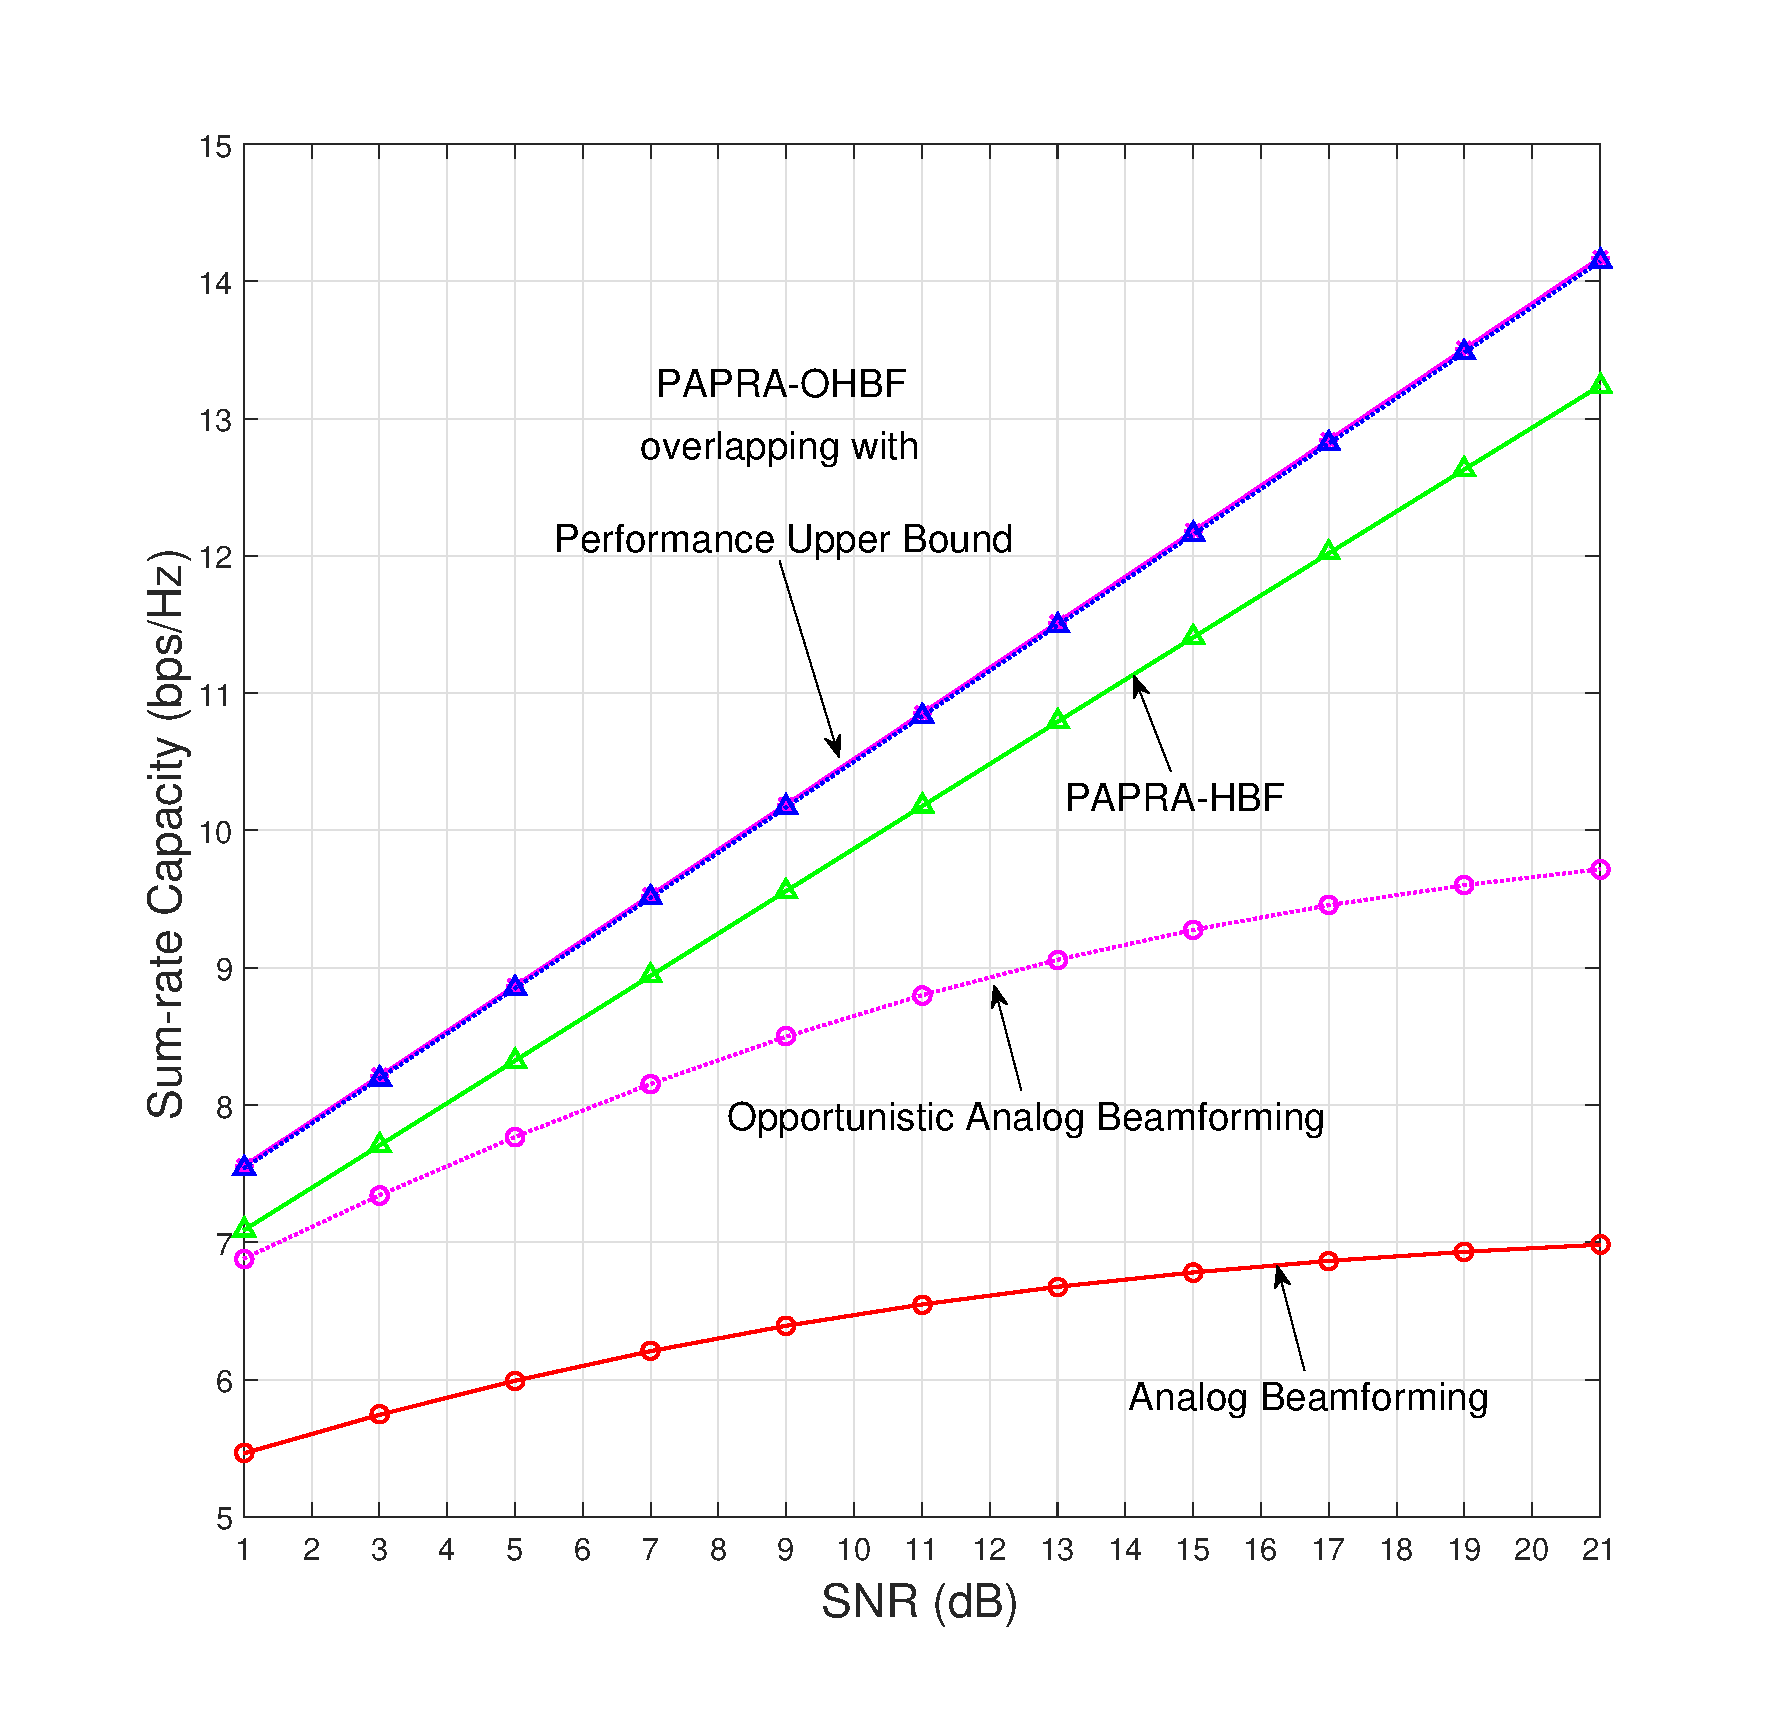
\includegraphics[width=3.8in,height=3in]{Figure/SpectralEffWithSelection2.eps}
 	\caption{Comparison of Sum-rate capacity for opportunistic schemes.}\label{fig:SpectralEffWithSelection}
    \end{center}
\end{figure}

Next, we investigate the performance provided by opportunistic hybrid beamforming. Inspection of Fig.~\ref{fig:SpectralEffWithSelection} shows that PAPRA-OHBF can achieve the optimal performance upper bound. Interestingly, as Fig.~\ref{fig:SpectralEffWithSelection} indicates the improvement above is partially attributed to the additional beamforming gain provided by opportunistic analog beamforming.

\begin{figure}[ht]
	\begin{center}
	\includegraphics[width=3.8in,height=3in]{Figure/MultiuserGain2.eps}
	\caption{Sum-rate capacity as a function of number of active users.}\label{fig:MultiuserGain}
    \end{center}
\end{figure}


Finally, we study the multiuser gain provided by opportunistic scheduling. By varying the number of active users, we investigate the sum-rate capacity improvement. Fig.~\ref{fig:MultiuserGain} shows that PAPRA-OHBF can significantly benefit from the increase of active users as the number of active users grows from $6$ to $20$. However, the benefit of having more active users diminishes as the number of active users increases beyond $30$. In contrast, the non-opportunistic analog beamforming is not capable of reaping multiuser gains. As a result, the curve labelled ``Analog Beamforming" does not change much with the number of active users.

\section{Conclusion}
In this work, we have developed PAPR-aware BDMA scheme for mmWave massive MIMO systems by jointly performing hybrid analog-digital precoding and user-beam scheduling. First, we have modeled the analog-digital precoder design as a convex optimization problem with explicit PAPR constraints. Simulation results have confirmed that the proposed BDMA scheme with optimized precoders can achieve better sum-rate capacity at a lower PAPR than the conventional clipping technique. Furthermore, in contrast to the conventional hybrid design that performs interference cancellation through digital precoding only, the proposed scheme is capable of suppress multiuser interference by scheduling users whose transmit array response vectors are close to be orthogonal. To efficiently schedule users with the least interference, we develop a greedy algorithm to opportunistically select users. Simulation results have demonstrated the good sum-rate performance of the proposed PAPR-aware BDMA scheme.

% references section
\bibliography{BDMAref}
\bibliographystyle{IEEEtran}
\end{document}


